\section{QuickDough Framework}\label{sec:framework}

\subsection{System Context}
This work assumes a hybrid computing architecture with a host processor and a FPGA accelerator, where the processor handles tasks not-well suited to FPGAs such as providing the OS environment and the end user GUI and FPGA focuses on computation intensive kernels.

Figure \ref{fig:typical-FPGA-accelerator} shows a typical FPGA acceleration architecture and all the experiments in this work sticked to it. In this system, FPGA accelerator is attached to the system bus and it could access main memory through the bus. Inner the FPGA accelerator, there are a
group of data buffers, an acceleration control block(Acc Ctrl), and the computation core. Data buffers are employed to store input data, output data and even temporary data of the computation core. The Acc Ctrl block receives computation start signal from CPU and then triggers the computation core when the input data is ready. Also it sends computation done signal back to interrupt CPU for data collection when the computation core completes. The computation core is a hardware structure customized for the application compute kernel, which is supposed to be fast.  

\begin{figure}[H]
    \center{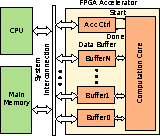
\includegraphics[width=0.5\linewidth]{typical-FPGA-accelerator}}
    \caption{A Typical FPGA Acceleration Architecture}
    \label{fig:typical-FPGA-accelerator}
\end{figure}

\subsection{QuickDough}
Based on the typical FPGA acceleration architecture, a rapid FPGA acceleration framework is developed as presented in Figure \ref{fig:framework}. Basically, it starts from HW/SW partition so that the application compute kernel can be extracted. The extracted kernel can further be transformed to data flow graph (DFG), which is preferred to be used in CGRA compilation. There are already intensive research on both, which could help us to automate the processing. Currently, we just manually perform the HW/SW partition and DFG transformation in our preliminary research stage. 

Afterwards, the design flow is split into two paths. The path on top half is basically a conventional software compilation flow except that we need to replace the compute kernel with CPU-FPGA accelerator communication drivers to manage the FPGA accelerator as an IO device. 

The path on the bottom half is esentially the hardware design flow. Given the application compute kernel, the SCGRA optimizer is supposed to decide the optimal DFG size and corresponding SCGRA configuration. However, we haven't got a systematic solution for the optimizer yet and we will just choose two SCGRA configuration as an example to show the benefits of the SCGRA based acceleration framework. After this step, if the required SCGRA configuration happens to be in the SCGRA library, then the SCGRA compiler could generate the FPGA bitstream directly. If not, corresponding SCGRA HDL code will be generated automatically based on the pre-defined template, and the HDL model is further implemented on the target FPGA device. Then the implementation result is added to the SCGRA library. Finally, SCGRA compiler will handle the scheduling and bitstream generation. Through the design iterations of an application or even across a whole application domain, it is possible that a single hardware implementation meets the design goal. While SCGRA compilation can be done around a minute, the design productivity can be improved significantly. 

\begin{figure}[H]
    \center{\includegraphics[width=0.95\linewidth]{framework}}
    \caption{QuickDough Framework}
    \label{fig:framework}
\end{figure}

